\documentclass[a4paper,12pt]{article}
\usepackage{stdtemplate}

\title{\vspace{-50pt}\bfseries{\Large{CSC373 Algorithms}}\vspace{-30pt}}
\author{\normalfont{Jonah Chen}}
\date{}
\begin{document}
\maketitle
\tableofcontents
\sffamily
\section{Divide and Conquer}
\begin{itemize}
    \item Divide and Conquer algorithm:
    \begin{enumerate}
        \item Divide problem of size $n$ into $a$ smaller subproblems of size $n/b$ each
        \item Recursively solve each subproblem
        \item Combine the subproblem solutions into the solution of the original problem
    \end{enumerate}
    \item Runtime: $T(1)=c$ and $T(n)=a T(n/b) + cn^d$ for $n>1$
    \item Master Theorem: $T(n)$ depends on relation between $a$ and $b^d$. \begin{equation}
        \begin{cases}
            a<b^d: T(n)=\Theta(n^d)\\
            a=b^d: T(n)=\Theta(n^d\log n)\\
            a>b^d: T(n)=\Theta(n^{\log_b a})
        \end{cases}
    \end{equation}
    \begin{itemize}
        \item Note that the running time does not depend on the constant $c$
        \item In many algorithms $d=1$ (combining take linear time)
    \end{itemize}
    \item Examples:
    \begin{itemize}
        \item Merge sort --- sorting array of size $n$ ($a=2,\,b=2,\,d=1\rightarrow a=b^d$) so $T(n)=\Theta(n\log n)$
        \item Binary search --- searching sorted array of size $n$ ($a=1,\,b=2,\,d=0\rightarrow a=b^d$) so $T(n)=\Theta(\log n)$
    \end{itemize}
\end{itemize}
\subsection{Karatsuba Multiplication}
\begin{itemize}
    \item \bluebf{Add} two binary $n$-bit numbers naively takes $\Theta(n)$ time
    \item \bluebf{Multiply} two binary $n$-bit numbers naively takes $\Theta(n^2)$ time
    \item Divide and Conquer approaches \begin{enumerate}
        \item Multiply $x$ and $y$. We can divide them into two parts\begin{align}
            x &= x_1\cdot 2^{n/2} + x_0\\
            y &= y_1\cdot 2^{n/2} + y_0\\
            x\cdot y &= x_1\cdot y_1\cdot 2^n + (x_1\cdot y_0 + x_0\cdot y_1)\cdot 2^{n/2} + x_0\cdot y_0 \label{eq:mul}
        \end{align}
        \begin{itemize}
            \item $T(n)=4T(n/2)+cn; T(1)=c$
            \item $a=4,b=2,d=1$ Master Theorem case 3, $T(n)=\Theta(n^{\log_2 4})=\Theta(n^2)$.
            \item This is the same complexity of the naive approach, making this approach useless.
        \end{itemize}
        
        \item Reconsider \eqref{eq:mul}, we may rewrite $(x_1\cdot y_0+x_0\cdot y_1)$ as $(x_1+x_0)\cdot(y_1+y_0)-x_1\cdot y_1-x_0\cdot y_0$
        \begin{equation}
            x\cdot y = x_1\cdot y_1\cdot 2^n + ((x_1+x_0)\cdot(y_1+y_0)-x_1\cdot y_1-x_0\cdot y_0)\cdot 2^{n/2} + x_0\cdot y_0
        \end{equation}
         
        \begin{itemize}
            \item $T(n)=3T(n/2)+cn; T(1)=c$
            \item $a=3,b=2,d=1$, Master Theorem case 3, $T(n)=\Theta(n^{\log_2 3})=\Theta(n^{\log_2 3})\approx\Theta(n^{1.585})$
            \item Minor issue: a carry may increase $x_1+x_0$ and $y_1+y_0$ to $\frac{n}{2} + 1$. We can easily prove this by isolating the carry bit and reevaluating the complexity.
        \end{itemize}
    \end{enumerate}
    \item To deal with integers which doesn't have a power of 2 number of bits, we can pad the numbers with 0s to make them have a power of 2 number of bits. This may at most increase the complexity by 3x.
    \item 1971: $\Theta(n\cdot\log n\cdot \log\log n)$
    \item 2019: Harvey and van der Hoeven $\Theta(n\log n)$. We do not know if this is optimal.
\end{itemize}
\subsection{Strassen's MatMul Algorithm}
\begin{itemize}
    \item Let $A$ and $B$ be two $n\times n$ matrices (for simplicity $n$ is a power of 2), we want to compute $C=AB$.
    \item The naive approach takes $\Theta(n^3)$ time.
    \begin{enumerate}
        \item Divide $A$ and $B$ into $4$ submatrices of size $\frac{n}{2}\times\frac{n}{2}$ each
        \begin{equation}
            A = \begin{bmatrix}
                A_{1} & A_{2}\\
                A_{3} & A_{4}
            \end{bmatrix}.
        \end{equation}
        Then, $C$ can be calculated with
        \begin{align}
            C_1 &= A_1B_1 + A_2B_3\\
            C_2 &= A_1B_2 + A_2B_4\\
            C_3 &= A_3B_1 + A_4B_3\\
            C_4 &= A_3B_2 + A_4B_4
        \end{align}
        \begin{itemize}
            \item $T(n)=8T(n/2)+cn^2; T(1)=c$
            \item $a=8,b=2,d=2$, case 3 $T(n)=\Theta(n^{\log_2 8})=\Theta(n^3)$
        \end{itemize}
        \item \textbf{Idea:} Compute $C_1,C_2,C_3,C_4$ with only $7$ multiplications, not 8.
        \begin{align}
            M_1 &= (A_2-A_4)(B_3+B_4)\\
            M_2 &= (A_1+A_4)(B_1+B_4)\\
            M_3 &= (A_1-A_3)(B_1+B_2)\\
            M_4 &= (A_1+A_2)B_4\\
            M_5 &= A_1(B_2-B_4)\\
            M_6 &= A_4(B_3-B_1)\\
            M_7 &= (A_3+A_4)B_1
        \end{align}
        With these we can compute $C_1,C_2,C_3,C_4$ with only additions of the $M$ matrices.
        \begin{align}
            C_1 &= M_1+M_2-M_4+M_6\\
            C_2 &= M_4+M_5\\
            C_3 &= M_6+M_7\\
            C_4 &= M_2-M_3+M_5+M_7
        \end{align}
        \begin{itemize}
            \item $T(n)=7T(n/2)+cn^2; T(1)=c$
            \item $a=7,b=2,d=2$, case 3 $T(n)=\Theta(n^{\log_2 7})=\Theta(n^{\log_2 7})\approx\Theta(n^{2.807})$
        \end{itemize}
    \end{enumerate}
    \item If $n$ is not a power of 2, we zero-pad the matrices to have $n$ as a power of two. This may increase the complexity by at most a factor of 7.
\end{itemize}

\subsection{Median of Unsorted Arrays}
\begin{itemize}
    \item For an unsorted array $A$, we can find the average, max, min, sum, etc. in linear time.
    \item The trivial algorithm is to sort $A$ then get the median. That takes $O(n\log n)$ time.
    \item We will solve a more general problem: Find the $k^{th}$ smallest element in $A$. (e.g. $A=5,2,6,7,4$, $\mathrm{Select}(A,1)=2, \mathrm{Select}(A,4)=6$)
    \item if $|A|=1$, then return $A[1]$. Otherwise find a splitter $s$ in arbitrary element of $A$. Partition $A$ into $A^+$ and $A^-$, then divide 
    \item $T(n)=T(\max(|A^-|,|A^+|))+cn=T(\max(i-1,n-i))+cn$.
    \item Worst case: $T(n)=T(n-1)+cn=\Theta(n^2)$
    \item Best case: $T(n)=T(n/2)+cn=\Theta(n)$. Suppose $b>1$, by the Master Theorem $T(n)=T(n/b)+cn=\Theta(n)$.
\end{itemize}

We define $s$ is a good splitter if $s$ is greater than $1/4$ of the elements of $A$ and less than $1/4$ of the elements of $A$. We can make the following observation:
\begin{enumerate}
    \item With this splitter, we will reduce the size to at most $3n/4$.
    \item Half the elements are good splitters.
\end{enumerate}

We should select splitter $s$ uniformly at random.
\begin{itemize}
    \item $P(\text{splitter is good})=\frac{1}{2}$
    \item $P(\text{splitter is bad})=\frac{1}{2}$
    \item We can show that the expected number of trials (splitter selections) until obtaining a good splitter is 2.
\end{itemize}
\subsubsection{Expected Runtime}
\begin{equation}
    \underbrace{n_0\to n_1\to n_2}_{\text{Phase 0, size}\leq n}\to \underbrace{n_3\to n_4}_{\text{Phase 1, size}\leq \frac{3}{4}n}\to \underbrace{n_5\to n_6}_{\text{Phase 2, size}\leq \frac{3}{4}^2 n}\to\dots
\end{equation}
\begin{itemize}
    \item Phase $j$: input size $\leq(\frac{3}{4})^j\,n$
    \item Random variable $y_j = $\# of recursive calls in phase $j$. Note that $E[y_j]=2$.
    \item Random variable $x_j = $\# of steps to all the recursive calls in phase $j$.
    \item Total number of steps is $x=x_0+x_1+x_2+\dots$.
    \item We can compute $E[x]=E[x_0]+E[x_1]+E[x_2]+\dots$.
    \begin{align}
        x_j&\leq c y_j \frac{3}{4}^j n\\
        E[x_j]&\leq c E[y_j] \frac{3}{4}^j n\leq 2c\frac{3}{4}^j n\\
        E[x]&=\sum_j E[x_j]\leq \sum_{j=1}^\infty 2c\frac{3}{4}^j n=\frac{2c}{1-\frac{3}{4}}n=8cn=\Theta(n)
    \end{align}
\end{itemize}

\subsubsection{Deterministic Algorithm}
\begin{itemize}
    \item If $|A|\leq 5$ then we sort $A$ and return the $k^{th}$ smallest.
    \item Otherwise, partition $A$ into $n/5$ groups of size $5$ each, then find the median of each group (constant time) and store in list $M$. This takes linear time.
    \item Select the median of $M$ with the Select algorithm, this is a good splitter.
    \item the worst case running time is $T(n)=T(\lceil\frac{n}{5}\rceil)+T(\lfloor{\frac{3n}{4}}\rfloor)+cn$.
    \item This recursive relation cannot be solved by the Master Theorem. We can prove using induction that $T(n)<20cn$.
\end{itemize}
\redbf{Question: Why groups of 5?}
\begin{itemize}
    \item With groups of 5, the total size of subproblems: $\frac{n}{5}+\frac{3n}{4}=\frac{19n}{20}<n$
    \item With groups of 3, the total size of subproblems: $\frac{n}{3}+\frac{3n}{4}=\frac{13n}{12}>n$, not sufficient.
    \item So group size of $5,7,9,11,\dots$ would also work.
\end{itemize}

\section{Closest Pair of Points}
\begin{itemize}
    \item Problem: Given a set of $n$ points, find the pair of points that are the closest in $O(n\log n)$.
\end{itemize}
\subsection{Closest Pair in 2D}
\begin{itemize}
    \item Divide: points roughly in half by drawing vertical line on midpoint
    \item Conquer: Find closest pair on each half, recursively.
    \item Combine: Find the closest pair $(p,q)$, $p\in L$, $q\in R$. However, there may be $\Theta(n^2)$ pairs.
\end{itemize}
\begin{itemize}
    \item Claim: Let $p=(x_p,y_p)\in B_L,q=(x_q,y_q)\in B_R$ with $y_p\leq y_q$. If $d(p,q)<\delta$ then there are at most \bluebf{six} other points (x,y) in $B$ such that $y_p\leq y\leq y_q$.
    \item Proof:
    \item $S_L=\{p'=(x,y):p'\neq p\in B_L\land y_p\leq y\leq y_q\}$ (other points on the left of the middle)
    \item $S_R=\{p'=(x,y):p'\neq q\in B_R\land y_p\leq y\leq y_q\}$ (other points on the right of the middle)
    \item Assume by contradiction that $|S_L\cup S_R|\geq 7$. WLOG assume $|S_L|\geq 4$.
    \item In a $\delta\times\delta$ square there are at least $4+1=5$ points. Divide the square into 4 smaller squares, by Pigeonhole Principle, there is a square with at least 2 points, whose distance is at most $\delta/\sqrt2$. This contradicts the assumption that the closest pair on the left is at most $\delta$.
\end{itemize}
\begin{itemize}
    \item Then, we can sort everything in the $y$ axis, and check the next seven points by the $y$ coordinate for the minimum distance. This takes linear time.
    \item We only need to modify the combine step in the algorithm so it's $\Theta(n)$ runtime.
\end{itemize}

\begin{algorithm}
\caption{Closest Pair in 2D}
\begin{algorithmic}[1]
\Procedure{ClosestPair}{$P$}
\State $P_x:=\text{the list of points in }P\text{ sorted by x-coordinate}$
\State $P_y:=\text{the list of points in }P\text{ sorted by y-coordinate}$
\EndProcedure
\Procedure{RCP}{$P_x,P_y$}
\If{$|P_x|\leq 3$}
\Return{$\text{brute force}(P_x)$}
\EndIf
\State $L_x:=\text{the first half of }P_x;R_x:=\text{the second half of }P_x$
\State $m:=(\text{max x-coordinate of }L_x+\text{min x-coordinate of }R_x)/2$
\State $L_y:=\text{sublist of }P_y\text{ with points in }L_x$
\State $R_y:=\text{sublist of }P_y\text{ with points in }R_x$
\State $(p_L,q_L):=\text{RCP}(L_x,L_y);(p_R,q_R):=\text{RCP}(R_x,R_y)$
\State $\delta:=\min\{d(p_L,q_L),d(p_R,q_R)\}$
\If {$\delta=d(p_L,q_L)$}
\State $p:=p_L;q:=q_L$
\Else
\State $p:=p_R;q:=q_R$
\EndIf
\State $B:=\text{sublist of }P_y\text{ with points in }[m-\delta,m+\delta]$
\Foreach {$p$ in $B$}
\Foreach {next seven $q$ after $p$ in $B$}
\If {$d(p,q)<d(p^*,q^*)$} $(p^*,q^*):=(p,q)$
\EndIf
\EndForeach
\EndForeach
\EndProcedure
\end{algorithmic}
\end{algorithm}
\begin{itemize}
    \item So $T(n)=2T(\frac{n}{2})+cn$, which is $O(n\log n)$.
\end{itemize}

\section{Greedy Algorithms}
\begin{itemize}
    \item There is an optimization problem: given an input, find a solution that minimize/maximize an objective function $f$ under some constraint.
    \item Build the solution incrementally in stages
    \item At each stage, extend the solution greedily and irrevocably.
    \item For some problems this gives optimal solutions (i.e. MST), but for other problems it does not.
    \item The order of the stages is very important.
\end{itemize}

\subsection{Interval Scheduling}
\begin{itemize}
    \item Input: $n$ intervals, with interval $j$ starts at time $s_j$ and finishes at time $f_j$.
    \item Output: maximum-size set of intervals that do not overlap
    \item Naive algorithm is to try each subset of $n$ intervals by brute force $O(2^n)$, way too slow.
    \item Greedy algorithm sorts interval in some order, then if it doesn't overlap then add it to the solution.
    \item \redbf{What order gives the biggest feasible set?}
    \begin{enumerate}
        \item Increasing start time: $s_j$
        \item Increasing finish time: $e_j$
        \item Shortest interval: $e_j-s_j$
        \item Fewest conflicts
    \end{enumerate}
    \item The question is which one is optimal? Option 1 has a clear counterexample with one very long interval that overlaps each other interval. Option 3 is also not optimal using a short interval between two long interval. Option 4 is not optimal (not very clear counterexample).
    \item Option 2 is optimal. The intuition is that chosing these intervals first will leave the most time for the rest of the intervals.
    \item To find if the interval is compatible, we just need to check if the start time of the new interval is greater than the finish time of the latest scheduled interval.
\end{itemize}
\subsubsection{Proof of optimality}
\begin{itemize}
    \item Suppose for contradiction that this greedy algorithm is not optimal
    \item Say greedy selects interval $i_1,\dots,i_k$ sorted by increasing finish time.
    \item Suppose the optimal schedule $j_1,\dots,j_m$ has $m>k$ intervals, and sort by increasing finish time. Consider an optimal schedule that can match the greedy $j_1=i_1,\dots,j_r=i_r$ for the greatest possible $r$.
    \item By the nature of the greedy algorithm, then $i_{r+1}$ finishes the earliest amongst the compatible intervals remaining. So consider the schedule $S:i_1,\dots,i_r,\mathbf{i_{r+1}},j_{r+2},\dots,j_m$. 
    \item This is also optimal (contains $m$ intervals) but matches the greedy algorithm by one more position. This is a contradiction.
\end{itemize}

\subsection{Interval Partitioning}
\begin{itemize}
    \item Motivation: given a set of lecture time intervals, schedule them into as few classrooms as possible.
    \item Input: $n$ intervals, interval $j$ starts at $s_j$ and finishes at $f_j$.
    \item Output: group interval into fewest partitions such that intervals in each partition are compatible.
    \item An idea is to find the maximum set of compatible intervals using the previous algorithm. This doesn't work.
    \item We can try the same orders as the previous problem, but only earliest start time is optimal in this case.
    \item To implement it efficiently, we will use a heap with increase-key operation.
\end{itemize}
\subsubsection{Proof of optimality}
\begin{itemize}
    \item We define the \bluebf{depth} at time $t$ as the number of intervals that contain time $t$. The \bluebf{maximum depth} $d_{max}$ is the maximum depth over all times.
    \item Clearly, the number of partitions needed is at least $d_{max}$. We will show that this greedy algorithm create only $d_{max}$ partitions.
    \item Let $d$ be the number of partition the greedy algorithm opened.
    \item Partition $d$ was created because there was an interval $j$ that overlaps with some previously scheduled interval in each of the $d-1$ other partitions.
    \item This means that for $d-1$ intervals, their start times are all before $s_j$ and their finish times are all after $f_j$ (otherwise $j$ must be compatible). Hence, the depth at $s_j$ is exactly $d$.
    \item Thus, $d_{max}\geq d$ so the greedy algorithm is optimal.
    \item Warning: this proof rely on the fact that the start time
\end{itemize}

\subsection{Minimum Lateness Scheduling}
\begin{itemize}
    \item $n$ intervals: $1,2,\dots,n$, with each interval $j$ requires $t_j$ units of time and has deadline $d_j$.
    \item The lateness of an interval is $l_j=\max\{0,f_j-d_j\}$
    \item Output the schedule that minimizes the maximum lateness $L=\max_jl_j$.
    \item Fact 1: there is an optimal schedule with no gaps.
    \item The naive algorithm is to try all possible schedules, which is $O(n!)$.
    \item For greedy algorithm, we will sort intervals in this order
    \begin{enumerate}
        \item Shortest processing time, $t_j$
        \item Smallest slack first $d_j-t_j$
        \item Earliest deadline first $d_j$
    \end{enumerate}
    \item 1 and 2 are not optimal, and they have simple counterexamples with $n=2$.
    \item an \bluebf{inversion} is two intervals $i,j$ such that $d_i>d_j$ but $i$ is scheduled before $j$.
    \item \redbf{Note that in general:} Define inversion as a violation of what your order is, then prove that inversion is slightly worse or bad.
\end{itemize}
\subsubsection{Proof of optimality}
\begin{itemize}
    \item Observation 1: The greedy algorithm has no gaps.
    \item Observation 2: The greedy algorithm has no inversions.
    \item We will prove
    \item \bluebf{Claim 1}: If a schedule $S$ with no gaps has an inversion, then $S$ has a pair of inverted intervals that are adjacent.
    \item Suppose for contradiction that there is $S$ with an inversion but does not have adjacent intervals that are inverted. Then, $d_j<d_i\leq d_{i+1}\leq d_{i+2}\leq\dots\leq d_{j-1}\leq d_j$, so $d_j<d_j$ which is a contradiction.
    \item \bluebf{Claim 2}: All schedules with no gaps and no inversions have the same lateness
    \item Let $S$ and $S'$ be two distinct schedules with no gaps and no inversions
    \item Note $S$ and $S'$ differ only by the schedule of intervals with the same deadline
    \item Consider the intervals with the same deadline, they must be adjacent in both $S$ and $S'$. As a group, the maximum lateness of these intervals is the same because the group will finish at the same time.
    \item \bluebf{Claim 3}: Swapping adjacent inverted interval does not increase lateness and reduces the total number of inversions by one.
    \item Let $i$ and $j$ denote two adjacent inverted intervals in the schedule $S$. By swapping $i$ and $j$, we get a schedule $S'$ with one fewer inversion.
    \item Let $l$ and $l'$ be the lateness before/after swap. $\forall k\neq i,j, l_k=l'_k$.
    \item We know $d_i>d_j$ because it was an inversion. Thus, $l_j\geq l_j'$ and $l_j\geq l_i'$
    \item $l_j=f_j-d_j\geq f_i'-d_i=l_i'$
    \item Suppose by contradiction that the greedy schedule $S$ is not optimal.
    \item Let $S^*$ is the schedule with no gaps and fewest inversion.
    \item \textbf{Case 1:} $S^*$ has no inversion. By claim 2, this is contradiction.
    \item \textbf{Case 2:} $S^*$ has at least one inversion. By claim 1, it must have two inverted intervals that are adjacent. By claim 3, we can swap them to get a schedule with no greater lateness with one fewer inversion so it must be optimal. Then $S^*$ does not have the fewest inversions among all optimal schedules. This is also a contradiction.
\end{itemize}
\subsection{Huffman Code}
\begin{itemize}
    \item Given an alphabet $\Gamma$: a set of $n$ symbols
    \item You need to encode symbols using binary code. 
    \item Fixed length code requires $\lceil\log n\rceil$ bits per symbol.
    \item This is easy to decode, but this is not optimal
    \begin{itemize}
        \item ``e'': 12.7\% of letters in english
        \item ``z'': 0.07\% of letters in english
        \item We should give a shorter code to ``e'' than ``z''.
    \end{itemize}
    \item The goal is to find a code that minimize the length of text coding
    \item Variable length code can save space, but is harder to decode. Suppose $\Gamma=\{a,b,c\}$ and $a=1,b=01,c=010$. Then $0101$ is ambiguous as $bb$ or $ca$.
    \item A \bluebf{prefix code} is a code where no codeword is a prefix of any other. Scan from left to right until you see a codeword.
    \item Prefix code can be represented as a binary tree (edges are leaf), with the leaves as the symbols.
    \item The efficiently of a code is the weighted height of this tree, where the weight of a leaf is the probability of that symbol.
\end{itemize}
\subsection{Prefix Code Problem}
\begin{itemize}
    \item Input: A set of $\Gamma$ with their frequencies $f:\Gamma\to\R$ where $\sum_{x\in\Gamma}f(x)=1$
    \item Output: Binary tree $T$ representing the optimal prefix code for $\Gamma,f$
    \item Optimal Solution is a tree with the weighted average height $AD(T)$ of the tree is minimum.
    \item \textbf{Fact 1:} An optimal tree is a full binary tree, where each internal has two children.
    \item \textbf{Fact 2:} In an optimal tree $T$, $\forall x,y;f(x)<f(y)\implies \mathrm{depth}_T(x)\geq\mathrm{depth}_T(y)$.
    \item \textbf{Fact 3:} If $x,y$ have minimum frequency, then there is an optimal tree $T$ such that $x,y$ are siblings and are at max depth.
    \item \textbf{Huffman's Algorithm}: Combine the two smallest frequencies into a new symbol $z$ with frequency $f(z)=f(x)+f(y)$, and repeat recursively until there are only two symbol left, in which case we assign them $0$ and $1$.
\end{itemize}
\subsubsection{Proof of Optimality}
\begin{itemize}
    \item We will prove by induction. The base case for $n=2$ is trivial.
    \item Induction hypothesis: for all $\Gamma,f$ for $n-1$ symbols, the algorithm produces an optimal tree.
    \item Let $\Gamma,f$ be an alphabet with frequencies with $n$ symbols. Let $H$ be the tree produced by the algorithm.
    \item  The algorithm constructed by $H$ by: (1) replacing two symbols $x,y\in\Gamma$ of minimum frequency with a new symbol $z$, and
    \begin{align}
        \Gamma'&=(\Gamma\setminus\{x,y\})\cup\{z\}\\
        f'(\alpha)&=\begin{cases}
            f(x)+f(y),&\alpha=z\\
            f(\alpha),&\text{otherwise}
        \end{cases}
    \end{align}
    \item We know that $x,y$ are siblings (with parent $z$) in $H$
    \item Since $H'$ has $n-1$ symbols, $H'$ is optimal for $\Gamma',f'$
    \item We know $AD(H)=AD(H')+f(x)+f(y)$
    \item Now take an optimal tree $T$ for $(\Gamma,f)$ where $x,y$ are siblings. We know $T$ exists by fact 3.
    \item Let $T'$ be the tree constructed from $T$ by removing $x,y$ and replacing their parent with symbol $z$ (and $f(z)=f(x)+f(y)$)
    \item Clearly, $T'$ is a prefix code for $(\Gamma',f')$ with $AD(T)=AD(T')+f(x)+f(y)$
    \item We know $AD(T')\geq AD(H')$ as $H'$ is optimal for $(\Gamma',f')$ Thus, $AD(T)-f(x)-f(y)=AD(T')\geq AD(H')=AD(H)-f(x)-f(y)\implies AD(T)\geq AD(H)$. but $T$ is optimal so $H$ is optimal.
\end{itemize}
\subsection{Dijkstra's Single-Source Shortest Path Algorithm}
\begin{itemize}
    \item Input: A weighted directed graph $G=(V,E)$ with weights $w:E\to\R_+$ and a source vertex $s\in V$
    \item Output: Length of the shortest path from $s$ to every other node $t\in V$
    \item Suppose $R$ is a subset of nodes of $G$ that includes $s.$ A path $s\to v$ is a \bluebf{$R$-path} from $s\to v$ is restricted to contain only in $R$ before reaching $v.$
    \item At a high level, the algorithm maintains a set $R\subseteq V,$ (at the beginning $s$, and at the end $V$)
    \item The algorithm also contains $d(v)$ where
    \begin{enumerate}
        \item if $v\in R$, then $d(v)$ is the length of the shortest path from $s\to v.$ This is exactly what we want.
        \item if $v\in V\setminus R$, then $d(v)$ is the length of the shortest $s\to v$ $R$-path.
    \end{enumerate}
    \item The goal of the algorithm is to have $R$ contain all the nodes. In each iteration, the algorithm adds one more node from $R$ and maintains its properties.
    \item The algorithm will greedily choose the node $u\in V\setminus R$ with the minimum $d(u)$.
    \item We know that $d(u)$ is the length of the shortest $s\to u$ $R$-path. We will show that this is also the length of the shortest $s\to u$ path. If the claim is true, we can
    \begin{enumerate}[label=\alph*)]
        \item move $u$ to $R$ and still maintain property 1.
        \item update $d(v)$ for nodes in $V\setminus R$ to satisfy property 2.
    \end{enumerate}
    \item The proof of the claim is simple, suppose by contradiction that there is a shorter path $P$ with $len(P)<d(u).$ $P$ must cross from $R$ to $V\setminus R$ at least once. Let $v$ be the first node this $P$ reaches in $V\setminus R,$ so first section of $P,$ we denote $P_1$ from $s\to v$ is an $R$-path. As all the weights are non-negative, $len(P)\geq len(P_1)\geq d(v)\geq d(u),$ so $len(P)$ cannot be less than $d(u),$ which is a contradiction.
    \item Upon adding $u$ to $R,$ we gain more freedom for $R$-paths. For points in $V\setminus R,$ we can choose to retain the previous $R$-path or to use $u$ for the new $R$-path. Thus, for some $v\in V\setminus R,$
    \begin{itemize}
        \item if the shortest $R$-path does not contain $u,$ do nothing.
        \item if the shortest $R$-path contains $u,$ then the new $d(v)=d(u)+w(u,v)$. \begin{itemize}
            \item Note that $u$ must be the last node in the shortest $R$-path. Suppose there is another node $r\in R$ where $s\to u\to r\to v$ is shorter than $s\to u\to v.$
            \item Since $r\in R$ when $u$ was still in $V\setminus R,$ $d(r)$ must be the length of the shortest path of $R\setminus\{u\}.$ So in this case, the shortest path to $v:s\to r\to v$ doesn't require $u.$
        \end{itemize}
    \end{itemize}
    \item So for every $v\in V\setminus R,$ we update $d(v)\gets\min\{d(v),d(u)+w(u,v)\}.$
    \item \begin{algorithmic}[1]
        \Procedure{Dijkstra}{}
        \State $R\gets\{s\}$
        \State $d(s)\gets 0$
        for each nodes $v\neq s$ do if $(s,v)$ is an edge then $d(v)\gets w(s,v), p(v)\gets s$ else $d(v)\gets\infty,p(v)\gets Nil$
        \While{$R\neq V$}
            \State $u\gets$ node not in $R$ with the minimum $d(u)$
            \State $R\gets R\cup\{u\}$
            \Foreach{$v$ s.t. $(u,v)$ is an edge}
                \If{$d(v)>d(u)+w(u,v)$}
                    \State $d(v)\gets d(u)+w(u,v)$
                    \State $p(v)\gets u$
                \EndIf
            \EndForeach
        \EndWhile
        \EndProcedure
        \end{algorithmic}
    \item \redbf{Note} that the algorithm does not work with negative weights.
\end{itemize}
\section{Dynamic Programming}
\begin{itemize}
    \item DP works on problems that have the \bluebf{optimal substructure property,} i.e. optimal solution can be computed efficiently from the optimal solution of subproblems.
    \item The method is to break the problem down into subproblems, solve each subproblem only once and \redbf{store} the solutions.
    \item When solving a subproblem, we look up previously computed solutions instead of recomputing it.
    \item Storing the solution to subproblems is called \bluebf{memoization.}
    \item DP is \textbf{different} from divide and conquer because:
    \begin{itemize}
        \item Divide and conquer is a special case of dynamic programming where the subproblems that are solve \redbf{never overlap}, so there's no need for memoization to avoid recomputing some previously solved solution.
    \end{itemize}
\end{itemize}
\subsection{DAG Shortest Path (Toy Problem)}
\begin{itemize}
    \item Given some directed acyclic graph, find the shortest path from the root to any leaf.
    \begin{enumerate}
        \item The greedy algorithm is not optimal (very simple counterexample).
        \item Naive recursion works, but it is very slow.
        \begin{itemize}
            \item If each node has $k$ children, then $T(0)=c,T(n)=kT(n-1)+c$ then the runtime is $\Theta(k^n)$.
            \item Note that in naive recursion, we are solving the same subproblems over and over again. Dynamic programming will aim to solve this problem.
        \end{itemize}
        \item Dynamic programming. We can solve the problem by caching the solutions of the subproblems and in a bottom-up order rather than top-down. With \begin{align}
            \mathrm{COST}(i)\gets\min\{&\mathrm{COST}(\mathrm{nextup}(i))+\mathrm{costup(i)},\\&\mathrm{COST}(\mathrm{nextdown}(i))+\mathrm{costdown(i)}\}.
        \end{align}
        The cost of this approach is equal to the number of nodes, which is $\Theta(n^k).$
    \end{enumerate}
\end{itemize}
\subsection{Weighted Interval Scheduling}
\begin{itemize}
    \item In normal interval scheduling, every interval is of equal importance. So we want to schedule the maximum number of intervals.
    \item Now, each interval have a weight (as some jobs are more important than others), so we want to schedule a set of compatible intervals with the maximum total weight.
    \item Clearly, the greedy algorithm by earliest finish time is not optimal. Sorting by weight is not optimal either. There are obvious counterexamples. Actually, no greedy approaches will work.
\end{itemize}

\subsubsection{Dynamic Programming Approach}
\begin{itemize}
    \item We will sort the intervals by increasing finish time $f_1\leq f_2\leq\cdots\leq f_n.$
    \item The \textbf{predecessor} of interval $p[j]$ is the largest index $i$ such that $f_i\leq s_j.$ ($p[j]=0$ if interval $j$ has no predecessors) We can find $p[j]$ in $O(\log j)$ time by doing binary search.
    \item Let $S$ be the optimal subset of intervals (for intervals $\{1,\dots,n\}$)
    \item Consider the last interval $n,$ either
    \begin{enumerate}
        \item $n\notin S,$ then $S$ is optimal for intervals $\{1,\dots,n-1\}.$
        \item $n\in S,$ then $S=\{n\}\cup$ optimal subsets of intervals $\{1,\dots,p[n]\}.$
    \end{enumerate}
    \item $S$ is the best of case $1$ and case $2,$ (that with the highest total weight).
    \item For dynamic programming in general, we want to define our notation and subproblems \eqref{weighted_interval_subproblem} to reach the \bluebf{Bellman equation} \eqref{weighted_interval_bellman}.
    \begin{align}
        OPT(j)&=\text{ max weight for intervals in }\{1,\dots,j\}\label{weighted_interval_subproblem}\\
        OPT(j)&=\begin{cases}
            0 & \text{if }j=0\\
            \max\{\mathrm{OPT}(j-1),\mathrm{OPT}(p[j])+w[j]\} & \text{if }j>0
        \end{cases}\label{weighted_interval_bellman}
    \end{align}
    \item We can use a top-down approach with recursion
    \begin{algorithmic}[1]
        \Procedure{TopDown}{$w,s,f$}
        \State Sort the intervals $(w,s,f)$ by increasing finish time $f_1\leq f_2\leq\cdots\leq f_n.$
        \State Compute $p[j]$ for $j=1,\dots,n.$ using binary search for each $p[j].$
        \State Let $OPT$ be a global array of size $n+1$ where $OPT[0]=0$
        \State\Return TD-OPT($n$)
        \EndProcedure
        \Procedure{TD-OPT}{$j$}
        \If{$OPT[j]$ is not initialized}
            \State TD-OPT$[j]\gets\max\{\text{TD-OPT}(j-1),\text{TD-OPT}(p[j])+w[j]\}$
        \EndIf
        \State\Return $OPT[j]$
        \EndProcedure
    \end{algorithmic}
    \item However, a bottom up approach is preferred as it is more simpler and shows that you understand dynamic programming better.
    \begin{algorithmic}[1]
        \Procedure{BottomUp}{$w,s,f$}
        \State Sort the intervals $(w,s,f)$ by increasing finish time $f_1\leq f_2\leq\cdots\leq f_n.$
        \State Compute $p[j]$ for $j=1,\dots,n.$ using binary search for each $p[j].$
        \State Let $\mathrm{OPT}$ be an array of size $n+1$ where $\mathrm{OPT}[0]=0$
        \For{$j=1$ to $n$}
            \State $\mathrm{OPT}[j]\gets\max\{\mathrm{OPT}[j-1],\mathrm{OPT}[p[j]]+w[j]\}$
        \EndFor
        \State \Return $OPT[n]$
        \EndProcedure
    \end{algorithmic}
    \item The runtime of both approaches is $\Theta(n\log n)$ due to the sorting and binary search. The space complexity is $\Theta(n)$.
    \item \redbf{Warning}: We need to be careful with our implementation. If we do not store enough information, we will still be solve the same problem multiple times. For example, the following approach does not work. \begin{algorithmic}[1]
        \Procedure{NaiveRec}{$j$}
        \If{$j=0$}
            \State \Return 0
        \Else
            \State \Return $\max\{\mathrm{NaiveRec}(j-1),\mathrm{NaiveRec}(p[j])\}$
        \EndIf
        \EndProcedure
    \end{algorithmic}
    \item Notes on bottom up versus top down:
    \begin{itemize}
        \item Top down may be preferred when not all sub-solutions need to be computed on some inputs, and one does not need to think about the right order as much.
        \item Bottom up may be preferred when all sub-solutions will anyway need to be computed, and it is sometimes faster because it prevents the overhead of recursive calls.
    \end{itemize}
    \item One way of figuring out what subproblems to define is to think ``we already know what the optimal solution is, then what is needed to reach that.''
    \item We can modify the algorithm to return the actual set of intervals that are chosen. There are two ways of doing this.
    \begin{enumerate}
        \item Computing the optimal set \textbf{simultaneously} with the optimal weight.
        \begin{algorithmic}[1]
            \Procedure{BottomUp}{$w,s,f$}
            \State Sort the intervals $(w,s,f)$ by increasing finish time $f_1\leq f_2\leq\cdots\leq f_n.$
            \State Compute $p[j]$ for $j=1,\dots,n.$ using binary search for each $p[j].$
            \State Let $\mathrm{OPT}$ be an array of size $n+1$ where $\mathrm{OPT}[0]=0$
            \State Let $S$ be an array of size $n$ where $S[0]\gets\emptyset.$
            \For{$j=1$ to $n$}
                \State $\mathrm{OPT}[j]\gets\max\{\mathrm{OPT}[j-1],\mathrm{OPT}[p[j]]+w[j]\}$
                \If{$\mathrm{OPT}[j]>OPT[j-1]$}
                    \State $S[j]\gets S[p[j]]\cup\{j\}$
                \Else
                    \State $S[j]\gets S[j-1]$
                \EndIf

            \EndFor
            \State \Return $S[n]$
            \EndProcedure
        \end{algorithmic}
        \item Computing the optimal set \textbf{after} the optimal weight is computed.
        \begin{algorithmic}[1]
            \Procedure{GetSet}{$OPT,p$}
            \State Let $S$ be an empty set.
            \State $i\gets n$
            \While{$i>0$}
                \If{$OPT[i]=OPT[i-1]$}
                    \State $i\gets i-1$ \Comment{$S$ does not contain $i$}
                \Else
                    \State $S\gets S\cup\{i\}$ \Comment{$S$ does contain $i$}
                    \State $i\gets p[i]$ \Comment{$S$ does not contain $p[i]+1,\dots,i-1$}
                \EndIf
            \EndWhile
            \State \Return $S$
            \EndProcedure
        \end{algorithmic}
    \end{enumerate}
\end{itemize}

\subsection{Edit Distance}
\begin{itemize}
    \item Input of two strings of $X=x_1,\dots,x_m$ and $Y=y_1,\dots,y_n$. An ``operation'' is defined as a deletion of a character, or replacement of a character with another character.
    \item Some applications are spelling correction, DNA sequencing, plagiarism detection, etc.
    \item We will solve a generalization of the edit distance problem. We will allow the cost of each operation to be different. So, we will also have as input \begin{itemize}
        \item Cost $d(a)$ of deleting a character $a$.
        \item Cost $r(a,b)$ of replacing a character $a$ with a character $b$ with $r(a,b)=r(b,a)$ and the triangle inequality $r(a,c)\leq r(a,b)+r(b,c)$ holds for any $b.$
    \end{itemize}
    We would try to find the minimum total cost for matching $X$ and $Y.$
    \item Sometimes it is helpful to think of if you have the optimal solution, what is the last operation that was performed? Here, consider the last symbols $x_m$ and $y_n.$ There are three cases:
    \begin{enumerate}[label=(Case \Alph*)]
        \item Deleting $x_m$ and optimally match $x_1,\dots,x_{m-1}$ with $y_1,\dots,y_n.$
        \item Deleting $y_n$ and optimally match $x_1,\dots,x_m$ with $y_1,\dots,y_{n-1}.$
        \item Match $x_m$ with $y_n$ and optimally match $x_1,\dots,x_{m-1}$ with $y_1,\dots,y_{n-1}.$
    \end{enumerate}
    \item Let $E(i,j)$ be the edit distance between $x_1,\dots,x_i$ and $y_1,\dots,y_j.$ Then, the Bellman equation is \begin{align}
        A&=E(i-1,j)+d(x_i)\\
        B&=E(i,j-1)+d(y_j)\\
        C&=E(i-1,j-1)+r(x_i,y_j)\\
        E(i,j)&=\begin{cases}
            \min\{A,B,C\}&\text{if $i,j>0$}\\
            \sum_{k=1}^i d(x_k)&\text{if $i>0$ and $j=0$}\\
            \sum_{k=1}^j d(y_k)&\text{if $j>0$ and $i=0$}\\
            0&\text{if $i=j=0$}
        \end{cases}
    \end{align}
    \item \redbf{Make sure to remember the base cases!}\begin{algorithmic}[1]
        \Procedure {EditDistance}{$X,Y,d,r$}
        \State Let $E$ be an array of size $(m+1)\times(n+1)$ indexed from $0.$
        \State $E(0,0)\gets 0$
        \For{$i=1$ to $m$}
            \State $E(i,0)\gets E(i-1,0)+d(x_i)$
        \EndFor
        \For{$j=1$ to $n$}
            \State $E(0,j)\gets E(0,j-1)+d(y_j)$
        \EndFor
        \For{$i=1$ to $m$}
            \For{$j=1$ to $n$}
                \State $A\gets E(i-1,j)+d(x_i)$
                \State $B\gets E(i,j-1)+d(y_j)$
                \State $C\gets E(i-1,j-1)+r(x_i,y_j)$
                \State $E(i,j)\gets \min\{A,B,C\}$
            \EndFor
        \EndFor
        \State \Return $E(m,n)$
        \EndProcedure
    \end{algorithmic}
    \item This algorithm is $O(mn).$ \redbf{When you need to compute an element (i.e. $E(m,n)),$ make sure its subproblems (i.e. $E(m-1,n-1),E(m,n-1),E(m-1,n)$) are computed!}
    \item To reconstruct the edits, we can obtain \begin{algorithmic}[1]
        \Procedure {RecoverPath}{$E,X,Y,d,r$}
        \State $Ops\gets\emptyset$
        \State $i\gets m; j\gets n$
        \While{$i>0\land j>0$}
            \If{$E(i,j)=d(x_i)+E(i-1,j)$}
                \State $Ops\gets Ops\cup\{\text{Delete $x_i$}\}$
                \State $i\gets i-1$
            \EndIf
            \If{$E(i,j)=d(y_j)+E(i,j-1)$}
                \State $Ops\gets Ops\cup\{\text{Delete $y_j$}\}$
                \State $j\gets j-1$
            \EndIf
            \If{$E(i,j)=r(x_i,y_j)+E(i-1,j-1)$}
                \State $Ops\gets Ops\cup\{\text{Replace $x_i$ with $y_j$}\}$
                \State $i\gets i-1$
                \State $j\gets j-1$
            \EndIf
        \EndWhile
        \EndProcedure
    \end{algorithmic}
    \item The recover path procedure is $O(m+n).$
\end{itemize}

\subsection{0-1 Knapsack}
\begin{itemize}
    \item The knapsack problem is: when given $n$ items, each with a value $v_i>0$ and weight $w_i>0$ and the knapsack can hold a weight $C.$ The goal is to find a subset $S$ of items with maximum total value such that the total weight of $S$ is at most $C.$
    \item 0-1 knapsack refers to you can either take an item or not take an item, nothing in between.
    \item Let $S$ be an optimal knapsack content for items $1,\dots,n$ and capacity $C.$
    \item There are two possible cases for the last item $n.$\begin{enumerate}
        \item If $n\notin S,$ then $S$ is optimal for items $1,\dots,n-1$ and capacity $C.$
        \item If $n\in S,$ then $S$ is optimal for items $1,\dots,n-1$ and capacity $C-w_n.$
    \end{enumerate}
    \item The subproblems we want to solve now have two parameters $n$ and $C,$ with $K(i,c)$ being the value of the optimal knapsack for $1,\dots,i$ and capacity $c.$
    \item The bellman equation is \begin{align}
        K(i,c)&=\begin{cases}
            0&\text{if $i=0$ or $c=0$}\\
            K(i-1,c)&\text{if $w_i>c$}\\
            \max\{K(i-1,c),K(i-1,c-w_i)+v_i\}&\text{if $w_i\leq c$}
        \end{cases}
    \end{align}
    \item We need to compute this by $0$ to $C$ first, then $0$ to $n.$
    \begin{algorithmic}[1]
        \Procedure{Knapsack}{$n,C,w,v$}
        \State For $c=0$ to $C$ do $K(0,c)\gets 0$\Comment{no items}
        \State For $i=0$ to $n$ do $K(i,0)\gets 0$\Comment{no capacity}
        \For{$i=1$ to $n$}
            \For{$c=1$ to $C$}
                \If{$c<w_i$}\Comment{item $i$ is too heavy}
                    \State $K(i,c)\gets K(i-1,c)$
                \Else\Comment{item $i$ can fit, take it or not}
                    \State $K(i,c)\gets \max\{K(i-1,c),K(i-1,c-w_i)+v_i\}$
                \EndIf
            \EndFor
        \EndFor
        \State \Return $K(n,C)$
        \EndProcedure
    \end{algorithmic}
    \item To find $S,$ we can backtrack from $K(n,C)$ to $K(0,0).$ \begin{algorithmic}[1]
        \Procedure{RecoverKnapsack}{$K,n,C,w,v$}
        \State $S\gets\emptyset;c\gets C;i\gets n$
        \While{$i>0$ and $c>0$}
            \If{$K(i,c)=K(i-1,c)$}\Comment{item $i$ is not in $S$}
                \State $i\gets i-1$
            \Else
                \State $S\gets S\cup\{i\}$
                \State $c\gets c-w_i$
                \State $i\gets i-1$
            \EndIf
        \EndWhile
        \State \Return $S$
        \EndProcedure
    \end{algorithmic}
    \item The time complexity is $O(nC).$ The space complexity is also $O(nC).$
    \item Question: is the running time polynomial in the \underline{input size}? \redbf{No!} because the number $C$ is \redbf{exponential in the number of bits} used to represent the input.
    \item This is \bluebf{pseudo-polynomial} because it is polynomial in the input values, not input size.
    \item The problem is NP-hard.
\end{itemize}
\subsubsection{Large Knapsack, Small Items}
\begin{itemize}
    \item Consider that instead of $C,w_1,\dots,w_n$ being small, we were told $v_1,\dots,v_n$ are small. Can we solve this problem in $O(nV)$ where $V=\sum v_i.$ Yes, with a different dynamic programming algorithm.
    \item Define our subproblems $K(i,v)$ to be the minimum capacity of a knapsack that can hold a total value of at least $v$ using items $1,\dots,i.$
    \item For item $i,$ either we should take $i$ to obtain value $v$ or we should not take $i.$
    \begin{itemize}
        \item If we do not choose $i,$ we need $K(i-1,v)$ capacity.
        \item If we do choose $i,$ we need $K(i-1,v-v_i)$ capacity.
    \end{itemize}
    \item The Bellman equation is \begin{align}
        K(i,v)&=\begin{cases}
            0&\text{if $v\leq0$}\\
            \infty&\text{if $v>0,i=0$}\\
            \min\{K(i-1,v),K(i-1,v-v_i)+w_i\}&\text{if $v>0,i>0$}
        \end{cases}
    \end{align}
    \item We should compute this array from $0$ to $V$ first, then $0$ to $n.$
\end{itemize}
\subsubsection{Approximation Algorithms}
\begin{itemize}
    \item Unless $P=NP,$ we cannot hope to solve knapsack in $O(poly(n,\log C,\log V)).$
    \item We can find a good approximate solution in polynomial time. $\forall\varepsilon>0$ we can get a solution that is at least $(1-\varepsilon)$-optimal, in time $O(poly(n,\log C,\log V,1/\varepsilon)).$
\end{itemize}

\subsection{Chain Matrix Multiplication}
\begin{itemize}
    \item Multiplying three matrices $D=ABC,$ then $D=(AB)C=A(BC).$ Although the answers are the same, the cost depends on the multiplication order.
    \item The problem is to find the optimal order of multiplication of a chain of matrices $A_1,\dots,A_n$ and each matrix has dimension $d_{i-1}\times d_i.$
    \item To multiply a $p\times q$ matrix by a $q\times r$ matrix, we obtain a $p\times r$ matrix with $pqr$ multiplications
    \item We define $m(i,j)$ as the minimum number of multiplication to compute $A_i\cdot A_{i+1}\cdot\cdots\cdot A_j.$
    \item Try all the ways to put the outer-level parentheses, then compute \begin{align}
        m(i,j)&=\begin{cases}
            0&\text{if $i=j$}\\
            \min_{i\leq k<j}\{m(i,k)+m(k+1,j)+d_{i-1}d_kd_j\}&\text{if $i<j$}
        \end{cases}
    \end{align}
    \item The naive recursive procedure takes $T(n)=\sum_{k=1}^{n-1}T(k)+T(n-k)+c.$ We can notice that both terms of the sum occur twice so simplify to \begin{align}
        T(n)&=2\sum_{k=1}^{n-1}T(k)+(n-1)c\\
        T(n+1)&=2\sum_{k=1}^{n-1}T(k)+n\\
        T(n+1)-T(n)&=2T(n)+c\\
        T(n+1)&=3T(n)+c\\
        T(n)&=\Theta(3^n)
    \end{align}
    \item This does not work. We can use dynamic programming to solve this problem in $O(n^3).$ We will compute from the bottom up, starting from chains of length $1$ to chains of length $n.$ \begin{algorithmic}[1]
        \Procedure{MatrixChainOrder}{$d_1,\dots,d_n$}
        \For{$i\gets 1$ to $n$}
            \State $m(i,i)\gets 0$
        \EndFor
        \For{$l\gets 1$ to $n-1$}
            \For{$i\gets 1$ to $n-l$}
                \State $j\gets i+l$
                \State $m(i,j)\gets\min_{i\leq k<j}\{m(i,k)+m(k+1,j)+d_{i-1}d_kd_j\}$
            \EndFor
        \EndFor
        \State \Return $m(1,n)$
        \EndProcedure
    \end{algorithmic}
\end{itemize}
\subsection{Bellman-Ford Single Source Shortest Paths}
\begin{itemize}
    \item We want to revisit the shortest paths problem. When the edge weights may be negative, Dijkstra's algorithm does not work. We want an algorithm that works with some negative edge weights.
    \item \redbf{Note that if the graph has a negative cycle, the problem makes no sense.}
    \item \textbf{Claim 1:} With no negative cycles, for every node $t\in V$ there is a shortest path that is \bluebf{simple} (i.e. contains no repeated nodes). Any cycle will have weight $\geq0,$ so just remote it and the path will not be any longer.
    \item Hence, for any node $t\in V,$ there is a shortest path with at most $n-1$ edges.
    \item For $t\neq s,$ consider an oracle that tells us the shortest path from $s$ to $t$ that contains $i$ edges $s\to\cdots\to u\to t.$ Then the shortest path from $s\to u$ has at most $i-1$ edges.
    \item We define our subproblems as $OPT(i,t)$ as the length of a shortest $s\to t$ path using \textbf{at most} $i$ edges. So, $OPT(i,t)=OPT(i-1,u)+w(u,t)$ for some $u\in V.$
    \item So, \begin{align}
        OPT(i,t)&=\begin{cases}
            0&\text{if $i=0$ and $t=s$}\\
            \infty&\text{if $i=0$ and $t\neq s$}\\
            \min_{u\in V}\{OPT(i-1,u)+w(u,t)\}&\text{if $i>0$}
        \end{cases}
    \end{align}
    Note that part of the $\min$ is the case where $u=t.$ In that case $w(t,t)=0$ so this case would be $OPT(i-1,t).$
    \item Then, $OPT(n-1,t)$ is the length of the shortest path from $s$ to $t.$ The naive implementation is $O(n^3).$ \begin{algorithmic}[1]
        \State $OPT(0,s)\gets0$
        \State for all $t\neq s,\,OPT(0,t)\gets\infty$
        \For{$i=1$ to $n-1$}
            \For{all $t\in V$}
                \State $OPT(i,t)\gets\min_{u\in V}\{OPT(i-1,u)+w(u,t)\}$
            \EndFor
        \EndFor
        \State \Return $OPT(n-1,t)$
    \end{algorithmic}
    \item We can improve this by not checking all the nodes, but only nodes that have an edge going \bluebf{into} $t$ as well as $t$ to itself. This is like reversing an adjacency list. Hence, instead of minimizing over all $u\in V,$ we only minimize over $u\in\{v\in V|w(u,t)<\infty\}.$ This way the runtime is $O(nm).$
    \item We do not have to store the matrix, which is $O(n^2)$ space. As each row only depends on the previous row, we can just store the two rows reducing the space complexity to $O(n).$
    \item To recover the path, we keep track of the current predecessor. Each time our path decreases, we update the predecessor.
\end{itemize}
\subsubsection{Detecting Negative Cycles}
\begin{itemize}
    \item \textbf{Claim 2:}\begin{align}
        \Big(\forall t\in V,\,OPT(k,t)=OPT(k-1,t)\Big)\implies\Big(\forall t\in V,\,OPT(k,t)=OPT(k+1,t)\Big).
    \end{align}
    \item Using the bellman equation, \begin{align}
        OPT(k+1,t)&=\min_{u\in V}\{OPT(k,u)+w(u,t)\}\\
        &=\min_{u\in V}\{OPT(k-1,u)+w(u,t)\}\\
        &=OPT(k,t).
    \end{align}
    \item Even if we don't care about negative cycles, this may help us stop early when we go through one iteration with no improvement.
    \item If $G$ has no negative cycle reachable from $s,$ \textbf{iff} $\forall t\in V,\,OPT(n,t)=OPT(n-1,t).$
    \item Proof $[\implies]:$ If there are no negative cycles reachable from $s,$ there exists a shortest path from $s$ to $t$ with at most $n-1$ edges. Hence, $OPT(n,t)=OPT(n-1,t).$
    \item Proof $[\impliedby]:$ Suppose $\forall t\in V,\,OPT(n,t)=OPT(n-1,t).$ Then for any $n'\geq n,OPT(n',t)=OPT(n-1,t).$ Suppose for contradiction that there is a negative cycle reachable from $s.$ Then, we can find a path from $s\to t$ for some $t$ in the negative cycle. We will repeat the negative cycle enough time so that $OPT(n',t)<OPT(n-1,t).$ This is a contradiction.
    \item Hence, to detect negative cycles we run Bellman Ford one extra time and check if $OPT(n,t)=OPT(n-1,t).$ If there is some $t\in V$ such that $OPT(n,t)<OPT(n-1,t),$ then there is a negative cycle reachable from $s.$
    \item \textbf{To detect all negative cycles}, we add a new node $s$ to the graph and connect it to all other nodes with weight $0.$ Then, we run Bellman Ford on this new graph. If there is a negative cycle it is reachable from $s.$
    \item \textbf{Claim 4:} Suppose that $OPT(n,t)\neq OPT(n-1,t)$ for some node $t.$ Then let $P$ be an $s\to t$ path of length $OPT(n,t)$ and with at most $n$ edges then \begin{enumerate}
        \item $P$ contains a cycle.
        \item Every cycle of $P$ has a negative length.
    \end{enumerate}
    \item $1$ is trivial, as the path has $n$ edges and $n+1$ nodes. By pigeonhole principle, there at least one node is included twice because $G$ only has $n$ nodes.
    \item Suppose $P=s\to\cdots\to v\to\cdots\to v\to\cdots\to t.$ Suppose by contradiction the path $v\to\cdots\to v$ has non-negative weight. Then, let $P'=s\to\cdots\to v\to\cdots\to t.$ The length of $P'$ is at most the length of $P$ but has at most $n-1$ edges. Hence, $OPT(n,t)\geq len(P')\geq OPT(n-1,t)$ which is a contradiction.
\end{itemize}
\subsection{Floyd-Warshall All-Pairs Shortest Paths}
\begin{itemize}
    \item Suppose we are given a graph $G=(V,E)$ with no negative length cycles. We want the shortest path from each node $s$ to each node $t.$ 
    \item If we use Bellman Ford, it will run in $O(n^2m)$ and if the graph is dense $m=O(n^2)$ then the runtime is $O(n^4),$ which is bad.
    \item $V=\{1,2,\cdots,n\}.$ We define $P$ as a $i\to^kj$ path if every intermediate node in $P$ is $\leq k.$ (i.e. $P=1\to 5\to 2\to 7$ is a $1\to^57$ path but not a $1\to^67$ path)
    \item Hence, we will define $OPT(i,j,k)$ as the length of the shortest (simple) $i\to^kj$ path. Consider the following two cases \begin{enumerate}
        \item $k$ is not an intermediate node of $P.$ Then, $OPT(i,j,k)=OPT(i,j,k-1).$
        \item $k$ is an intermediate node then $OPT(i,j,k)=OPT(i,k,k-1)+OPT(k,j,k-1).$
    \end{enumerate}
    \item The bellman equation is \begin{align}
        OPT(i,j,0)&=\begin{cases}
            0&\text{if }i=j\\
            w(i,j)&\text{if }i\to j\text{ is an edge}\\
        \end{cases}\\
        OPT(i,j,k)&=\min\{OPT(i,j,k-1),OPT(i,k,k-1)+OPT(k,j,k-1)\}
    \end{align}
    \begin{algorithmic}[1]
        \For{$i=1$ to $n$}
            \For{$j=1$ to $n$}
                \If{$i=j$}
                    \State $OPT(i,j,0)=0$
                \Else
                    \State $OPT(i,j,0)=w(i,j)$
                \EndIf
            \EndFor
        \EndFor
        \For{$k=1$ to $n$}
            \For{$i=1$ to $n$}
                \For{$j=1$ to $n$}
                    \If{$OPT(i,j,k-1)>OPT(i,k,k-1)+OPT(k,j,k-1)$}
                        \State $OPT(i,j,k)=OPT(i,k,k-1)+OPT(k,j,k-1)$
                    \Else
                        \State $OPT(i,j,k)=OPT(i,j,k-1)$
                    \EndIf
                \EndFor
            \EndFor
        \EndFor
    \end{algorithmic}
    \item The runtime complexity is $O(n^3).$ Naively, the space complexity is also $O(n^3),$ but note that row $k$ only depends on row $k-1,$ so we can reduce the space complexity to $O(n^2).$
    \item To recover the path, each node need to store for every source, what is the previous node in the shortest path.
\end{itemize}
\subsubsection{Transitive Closure Graph}
\begin{itemize}
    \item The \bluebf{transitive closure} of a graph $G^*=(V,E^*),$ where \begin{align}
        E^*=\{(u,v)|G\text{ has an edge from $u\to v$}\}.
    \end{align}
    \item To compute the transitive closure of $G(V,E),$ we can use Floyd Warshall after changing all edge weights to $i.$ If $OPT(u,v,n)\neq\infty\iff G$ has a $u\to v$ path $\iff G^*$ has an edge from $u\to v.$
    \item A better way is to modify the Floyd Warshall (replace $+$ with $\land$ and $\min$ with $\lor$)
\end{itemize}
\subsubsection{Detecting Negative Cycles}
\begin{itemize}
    \item \textbf{Claim 4:} If $G$ has a negative cycle, then $\exists u\in V,OPT(u,u,n)<0$ 
\end{itemize}

\section{Network Flow}
\begin{itemize}
    \item A \bluebf{flow network} $\mathcal F=(G,s,t,c)$ where $G=(V,E)$ is a directed graph and $s\in V$ is the start node and have no incoming edge, $t\in V$ is the terminal node and have no outgoing edge, and $c:E\to\R_+$ is the capacity function.
    \item A \bluebf{flow} $f:E\to\R$ that respects the following constraints:\begin{enumerate}
        \item $\forall\,e\in E,0\leq f(e)\leq c(e)$
        \item $\forall\,v\in V\setminus\{s,t\},\sum_{e\in E^+(v)}f(e)-\sum_{e\in E^-(v)}f(e)=0$
    \end{enumerate}
    \item The \bluebf{value} of a flow $f$ is $v(f)=f^{out}(s)=f^{in}(t).$
    \item The \textbf{max-flow problem} is: given a flow network $\mathcal F$ to find the flow $f$ with maximum $v(f).$
    \item Given a flow $f,$ the \bluebf{residual graph} is the graph $G_f=(V,E_f)$ where for each edge $(u,v)\in E,$ $E_f$ has at most two edges \begin{itemize}
        \item Forward edge: $e=(u,v)$ with residual capacity $c(e)-f(e)>0$
        \item Reverse edge: $e'=(v,u)$ with residual capacity $f(e')>0$) 
    \end{itemize}
    Note that if an edge is saturated, the edge is not included in $E_f.$
    \item An \bluebf{augmenting path} is a path $P$ in $G_f$ from $s$ to $t.$ The \bluebf{bottleneck} of $P$ is the smallest residual capacity of any edge in $P.$
    \item To augment $f,$ we can add the bottleneck $x$ of an augmenting path to $f$ to obtain $f'$ by \begin{itemize}
        \item For each forward edge of $P,$ increase the flow by $x.$
        \item For each reverse edge of $P,$ decrease the flow by $x.$
    \end{itemize}
    \item We will first argue that $v(f')>v(f).$ As there is no edge into $s,$ we only have forward edges from $s,$ then $v(f')=f'^{out}(s)=f^{out}(s)+x>v(f)$
    \item We also need to argue we do not violate the capacity constraints. This is trivial.
    \item Finally, we must argue that flow conservation is preserved. At each node $e,$ we must consider $4$ cases. \begin{enumerate}
        \item If $v$ is not on $P,$ then nothing changes.
        \item The edge entering $v$ and the edge leaving $v$ in the augmenting path $P$ are both forward edges. Then both $f^{out}(v)$ and $f^{in}(v)$ increase by $x.$
        \item If one is forward and one is reverse, then $f^{in}(v)$ and $f^{out}(v)$ are unchanged.
        \item If both are reverse, then both $f^{in}(v)$ and $f^{out}(v)$ decrease by $x.$
    \end{enumerate}
\end{itemize}
\subsection{Ford-Fulkerson Algorithm}
\begin{algorithmic}[1]
    \Procedure{FordFulkerson}{$\mathcal F=(G,s,t,c)$}
        \Foreach{edge $(u,v)$ of $G$} 
            \State $f(u,v)\leftarrow 0$
        \EndForeach
        \State construct $G_f$
        \While{$G_f$ has an $s\to t$ path}
            \State $P\gets$ any simple $s\to t$ path in $G_f$
            \State augment$(f,P)$
            \State update $G_f$
        \EndWhile
        \State \Return $f$
    \EndProcedure
\end{algorithmic}
\begin{itemize}
    \item First, assume edge capacities are integers. Note at every step, everything remains as integers. In every step, the flow increases by at least $1.$ An upper bound on the max flow is $C=\sum_{e\text{ leaving }s}c(e).$ Assume every node is reachable from $s,$ then an upper bound on the runtime $O((m+n)\cdot C).$ This is pseudo-polynomial time because $C$ can be large.
    \item To make the algorithm run in polynomial time, we can pick the augmenting path with the maximum bottleneck capacity.\begin{itemize}
        \item Using a modified Dijkstra's algorithm with a Fibonacci heap, we each iteration takes $O(m+n\log n)$ time.
        \item We can prove that this takes at most $O(m\log C)$ iterations. Hence, the total running time is $O(m^2\log C+mn\log n\log C).$
    \end{itemize}
    \item We can also pick the augmenting path with the minimum number of edges. \begin{itemize}
        \item Using BFS takes $O(m)$ time per iterations.
        \item We can prove at most $O(mn)$ iterations. Hence, the total running time is $O(m^2n)$.
    \end{itemize}
\end{itemize}
\subsection{Correctness of Ford-Fulkerson}
\begin{itemize}
    \item Given a network flow $\mathcal F=(G=(V,E),s,t,c),$ then $(A,B)$ is an \bluebf{$s$-$t$ cut} of $\mathcal F$ if $(A,B)$ is a partition of $V$ with $s\in A$ and $t\in B.$
    \item The \bluebf{cut capacity} of $(A,B)$ is $cap(A,B)=\sum_{e:A\to B}c(e).$
    \item \textbf{Claim:} For any flow $f$ and any $s$-$t$ cut $(A,B),$ then $v(f)=f^{out}(A)-f^{in}(A)$ where $f^{out}(A)=\sum_{e:A\to B}f(e)$ and $f^{in}(A)=\sum_{e:B\to A}f(e).$ The proof is trivial but tedious.
    \item \textbf{Claim:} For any flow $f$ and any $s$-$t$ cut $(A,B),$ then $v(f)\leq cap(A,B).$ The proof is $v(f)=f^{out}(A)-f^{in}(A)\leq f^{out}(A)=\sum_{e:A\to B}f(e)\leq\sum_{e:A\to B}c(e)=cap(A,B).$
    \item \textbf{Claim:} For any flow $f$ and any $s$-$t$ cut $(A,B),$ if $v(f)=cap(A,B)$ then $f$ is a max flow and $(A,B)$ is a \bluebf{min cut} (i.e. a cut with minimum cut capacity).
    \item Proof: Let $f^*$ be a max flow and $(A^*,B^*)$ be a min cut. Let $f$ be any flow and $(A,B)$ be any $s$-$t$ cut. Then, $v(f)\leq v(f^*)$ and $v(f)\leq v(f^*)\leq cap(A^*,B^*)\leq cap(A,B).$ If $v(f)=cap(A,B),$ then $v(f)=v(f^*)=cap(A^*,B^*)=cap(A,B).$ Thus, $f$ is a max flow and $(A,B)$ is a min cut. This is known as the \bluebf{max-flow min-cut theorem.}
    \item Now we are ready to prove that Ford-Fulkerson algorithm is correct. Let $f$ be the flow returned by the algorithm, and $G_f$ be the corresponding residual graph. Let $A$ be the set of nodes that are reachable from $s$ in $G_f$ and let $B=V\setminus A.$ Clearly, $(A,B)$ is an $s$-$t$ cut because $s\in A$ and $t\in B.$ Note that \begin{itemize}
        \item Let $u\in A$ and $v\in B.$ Suppose for contradiction that $f(u,v)<c(u,v)$ Then, $G_f$ will have an edge from $(u,v)$ so will an path from $s\to v.$ However, by definition $v$ is not reachable from $s$. This is a contradiction.
        \item We also know $f(v,u)=0.$ Suppose for contradiction $f(v,u)\neq 0.$ Then $G_f$ will have an reverse edge $(u,v)$ so $v$ is reachable from $s.$ However, by definition $v$ is not reachable from $s$. This is a contradiction.
    \end{itemize}
    By claim 2, \begin{align}
        v(f)&=f^{out}(A)-f^{in}(A)\\
        &=\sum_{u\in A,v\in B}f(u,v)-\sum_{u\in B,v\in A}f(v,u)\\
        &=\sum_{u\in A,v\in B}c(u,v)-0\\
        &=cap(A,B)
    \end{align}
    By max-flow min-cut, we know $f$ is a max flow. As a bonus, we also know $(A,B)$ is a min cut.
    \item \bluebf{Integrality Theorem:} If all the edge capacities are integers, $\exists$ an integral max flow $f$.
    \item Ford-Fulkerson algorithm can also be used to find the min cut
    \begin{algorithmic}[1]
        \Procedure{MinCut}{$\mathcal F$}
            \State $f\gets$ Ford-Fulkerson($\mathcal F$)
            \State compute residual graph $G_f$
            \State $A\gets\{\text{all nodes that are reachable from $s$ in $G_f$}\}$
            \State $B\gets V\setminus A$
            \State \Return $(A,B)$
        \EndProcedure
    \end{algorithmic}
\end{itemize}

\subsection{Bipartite Matching}
\begin{itemize}
    \item $G=(V,E)$ is an undirected graph. A \bluebf{matching} $M$ in $G$ is a subset of edges of $G$ such that no two edges share the same node.
    \item A \bluebf{maximal matching} is not a subset of another matching.
    \item A \bluebf{maximum matching} is a maximal matching that contains the greatest number of nodes.
\end{itemize}
A \bluebf{bipartite graph} is an undirected graph such that $G=(V,E)$ such that $V$ is partitioned into $X$ and $Y,$ and every $e\in E$ connects a node in $X$ to a node in $Y.$ It is also sometimes written as $G=[(X,Y),E].$ Reminder: an undirected graph $G$ is bipartite $\iff G$ has no odd cycle. Can determine if $G$ is bipartite in $O(m+n)$ using BFS or DFS.
\begin{itemize}
    \item Our problem is given a bipartite graph $G=(V,E)$ output the maximum matching of $G.$
    \item We can reduce this to the max-flow problem by turning $G=[(X,Y),E]$ into $\mathcal F=(G',s,t,c)$ by \begin{enumerate}
        \item Directing all edges of $G$ from $X$ to $Y.$
        \item Connect $s$ to each $x\in X$ and connect each $y\in Y$ to $t.$
        \item Assign a capacity of $1$ to each edge.
    \end{enumerate}
    \begin{algorithmic}[1]
        \Procedure{BipartiteMatching}{$G$}
        \State construct flow network $\mathcal F$ from $G$
        \State $f\gets\mathrm{MaxFlow}(\mathcal F)$
        \State $M_f\gets\{(x,y)|x\in X,y\in Y, f(x,y)=1\}$
        \State \Return $M$
        \EndProcedure
    \end{algorithmic}
    \item By the integrality theorem, $f$ is $0$ or $1$ on each edge.
    \item The running time of the algorithm is $O(mC).$ Here, $C=|X|=O(n),$ so it's $O(mn).$
    \item Now, we will show that $M$ is a matching and it is optimal.
    \item \textbf{Claim:} $\exists$ matching of size $k$ in $G\iff\exists$ integral flow of value $k$ in $\mathcal F.$
    \item $[\implies]$ Given a matching $M$ of size $k,$ construct $f(s,x)=f(x,y)=f(y,t)=1$ if $x\in X$ is matched with $y\in Y.$ As each $x$ is only matched with at most one $y$ and vise versa, $f(s,x)\leq1$ and $f(y,t)\leq1.$ Hence, this flow satisfies a capacity constraint.
    \item To show the flow conservation rules are satisfied, we can enumerate all six cases where it could fail and show they are impossible.
    \item $[\impliedby]$ Given an integral flow $f$ in $\mathcal F$ of value $k,$ we can construct a matching $M_f$ in $G$ of size $k$ by \begin{itemize}
        \item For each edge $(x,y)$ s.t. $f(x,y)=1,$ match $x$ with $y.$ 
        \item If this is a matching, there is a flow of $k$ from $s,$ and by flow conservation $k$ edges from $X$ to $Y$ must have flow $1,$ so the size of the matching is $k.$ 
        \item  By contradiction suppose this is not a matching. Then either $x_1,x_2\in X$ connects to $y\in Y$ then by flow conservation $f(y,t)\geq2$ which violates capacity constraint. Or, $x\in X$ connects to $y_1,y_2\in Y.$ Then $f(s,x)\geq2$ which also violate the capacity constraint.  
    \end{itemize}
    \item This shows that $M$ is an optimal matching because we found the max flow of $\mathcal F.$
\end{itemize}
\subsection{Min Vertex Cover}
\begin{itemize}
    \item Given an undirected graph $G=(V,E).$ A \bluebf{vertex cover} $V'\subseteq V$ is a subset s.t. every edge has at least one endpoint in $V'.$ A minimum vertex cover is a vertex cover of minimum size.
    \item In a general graph, finding a min vertex cover is NP-Complete, but we can have a polynomial time algorithm for bipartite graphs.
    \item \textbf{Claim:} for any matching $M$ in $G$ and any vertex cover $C$ of $G,$ then $|M|\leq|C|.$ The proofs follow from every edge in $M$ is covered by at least one node in $C$ and every node in $C$ is covered by at least one edge in $M.$
    \item \textbf{Claim:} For any matching $M$ in $G$ and any vertex cover $C$ of $G,$ if $M$ is a maximum matching, then $C$ is a minimum vertex cover. This follows straight from the inequality of the previous claim.
    \item \textbf{Claim:} If $G=[(X,Y),E]$ is a bipartite graph, then the size of the maximum matching is equal to the size of the minimum vertex cover. \redbf{This is not true for general graphs.} Consider a complete graph $K_3$ with three nodes $A,B,C.$ The maximum matching is size $1$ and the minimum vertex cover is size $2.$ \begin{itemize}
        \item Given a bipartite graph $G$ construct a flow network $\mathcal F$ as before. Let $f$ be the integral max flow in $\mathcal F$ from the Ford-Fulkerson algorithm, and let $G_f$ be the residual graph.
        \item Let $S$ be the nodes reachable from $s$ in $G_f,$ and $T=V\setminus S.$ $(S,T)$ is a min-cut with capacity of $cap(S,T)=v(f).$
        \item Consider the type of edges in $F$ from $S$ to $T:$\begin{enumerate}
            \item $s\to X\cap T,$ there are $|X\cap T|$ edges.
            \item $Y\cap S\to t,$ there are $|Y\cap S|$ edges.
            \item $\cancel{X\cap S\to Y\cap T},$ there are $0$ edges (we will show this later)
        \end{enumerate}
        \item $C=(X\cap T)\cup(Y\cap S)$ is a vertex cover of $G.$ We know $G$ has $4$ types of edges \begin{enumerate}
            \item $X\cap S\to Y\cap S$ is covered by nodes in $Y\cap S.$
            \item $X\cap T\to Y\cap T$ is covered by nodes in $X\cap T.$
            \item $X\cap T\to Y\cap S$ is covered by nodes in $X\cap T$ (and $Y\cap S$).
            \item $X\cap S\to Y\cap T$ contains no edges.
        \end{enumerate}
        \item Let $M$ be the matching corresponding to the flow $f$ \begin{align}
            |C|=|X\cap T|+|Y\cap S|&=|X\cap T|+|Y\cap S|=cap(S,T)=v(f)=|M|
        \end{align}
        So $|C|=|M|$ for some matching $M$ of $G$ so $C$ is a min vertex cover.
        \item Now we will show there are no edges from $X\cap S$ to $Y\cap T$. By contradiction let  $x\in X\cap S$ and $y\in Y\cap T$ where $G$ has edge from $x\to y$ In the residual graph, there is no edge from $x\to y.$ So, $f(x,y)=1.$
        \item As $x\in S,$ there is a path from $s\to x$ in $G_f.$ If the path is simple, then $f(s,x)=0$ so flow conservation is violated.
        \item With reverse edges in $G_f,$ a path $P:s\to x_1\to y_1\to\cdots\to x_k\to y_k\to x$ is possible where $y_1,\dots,y_k\in Y\cap S.$ Because $G_f$ has a reverse edge $y_k\to x,$ we know $f(x,y_k)=1.$ Also, $f(x,y)=1$ so the flow leaving $x$ is at least $2,$ which violates flow conservation.
    \end{itemize}
    \begin{algorithmic}[1]
        \Procedure{BipartiteVC}{$G=[(X,Y),E]$}
            \State construct flow network $\mathcal F$ from $G$
            \State $f\gets\mathrm{MaxFlow}(\mathcal F)$
            \State $S\gets\text{ nodes reachable from }s\text{ in }G_f$
            \State $T\gets V\setminus S$
            \State $VC\gets(X\cap T)\cup(Y\cap S)$
            \State \Return $VC$
        \EndProcedure
    \end{algorithmic}
    Running time is the same as max matching, $O(mn).$
\end{itemize}
\subsection{Hall's Theorem}
\begin{itemize}
    \item A \bluebf{perfect matching} in a bipartite graph $G=([X,Y],E)$ with $|X|=|Y|$ is a matching $M$ s.t. $M$ covers all nodes in $G.$
    \item Hall's theorem states that a bipartite graph $G=([X,Y],E)$ has a perfect matching iff $\exists X'\subseteq X$ s.t. $|X'|>|N(X')|.$
    \item $[\impliedby]$ is straightforward.
    \item $[\implies]$ Assume no perfect matching for $G$ exists. So, any matching $M$ will have $|M|<n/2.$ Let $R$ be a min vertex cover of $G$ so $|R|<n/2.$ Let $X'=X\setminus R$ then $|X'|>n/2.$ Then, $|X'|>n/2>|R|>|Y\cap R|.$ There is no neighbor of $X'$ in $Y\setminus R$ otherwise we can match them. Thus, $|N(X')|\leq|Y\cap R|<|X'|.$
    \item The contrapositive is also useful.
\end{itemize}
\subsection{Edge Disjoint Sets}

\section{Linear Programming}
\begin{itemize}
    \item Linear programming aims to minimize/maximize an objective function. The objective function is a linear combination of variables, subject to equality or inequality constraints (also linear combinations of variables).
    \item Many optimization problems can be formulated as linear programs. The main idea for us is how to recognize and formulate problems as linear programming problems.
\end{itemize}
\subsection{Examples}
Diet Problem:
\begin{itemize}
    \item We have $n$ types of food: $F_1,\dots,F_n,$ $m$ types of nutrients: $N_1,\dots,N_m,$ and each unit of food $F_j$ for $j\in\{1,\dots,n\}$ costs $c_j$ and provides $a_{ij}$ units of nutrient $N_i.$
    \item We must obtain at least $b_i$ units of nutrient $N_i$ for $i\in\{1,\dots,m\}.$
    \item Our goal is to minimize the cost of the food we buy.
    \item To formulate this problem as a linear programming problem, we select our \begin{itemize}
        \item \textbf{variables} as $x_1,\dots,x_n$ where $x_j$ is the amount of food $F_j$ in the diet. 
        \item \textbf{objective function} as $c_1x_1+\cdots+c_nx_n$ to be minimized.
        \item \textbf{constraints} as $a_{11}x_1+\cdots+a_{1n}x_n\geq b_1,$ $\cdots,$ $a_{m1}x_1+\cdots+a_{mn}x_n\geq b_m$ \redbf{and} $x_1,\dots,x_n\geq 0.$
    \end{itemize}
\end{itemize}
Profit Maximization Problem:
\begin{itemize}
    \item We can produce $n$ types of products $P_1,\dots,P_n$ and $m$ types of resources $R_1,\dots,R_m$ where each unit of product $P_j$ requires $a_{ij}$ units of resource $R_i$ and produces $c_j$ profit.
    \item You only have $b_i$ units of resource $R_i$ for $i\in\{1,\dots,m\}.$ We want to maximize the profit.
    \item To formulate this problem as a linear programming problem, we select our \begin{itemize}
        \item \textbf{variables} as $x_1,\dots,x_n$ where $x_j$ is the amount of product $P_j$ produced. 
        \item \textbf{objective function} as $c_1x_1+\cdots+c_nx_n$ to be maximized.
        \item \textbf{constraints} as $a_{11}x_1+\cdots+a_{1n}x_n\leq b_1,$ $\cdots,$ $a_{m1}x_1+\cdots+a_{mn}x_n\leq b_m$ and $x_1,\dots,x_n\geq 0.$
    \end{itemize}
\end{itemize}
Transportation Problem:
\begin{itemize}
    \item We have factories $F_1,\dots,F_k$ that manufacture the same product, and outlets $O_1,\dots,O_l$ that sell the product. Each factory $F_i$ has a supply $s_i$ and each outlet $O_j$ has a demand at least $d_j.$ The cost of shipping one unit of product from factory $F_i$ to outlet $O_j$ is $c_{ij}.$
    \item We want to minimize the total cost of shipping.
    \item To formulate this problem as a linear programming problem, we select our \begin{itemize}
        \item \textbf{variables} as $x_{ij}$ where $x_{ij}$ is the amount of product shipped from factory $F_i$ to outlet $O_j.$ 
        \item \textbf{objective function} as $\sum_i\sum_jc_{ij}x_{ij}$ to be minimized.
        \item \textbf{constraints} are $\sum_jx_{ij}=s_i$ for $i\in\{1,\dots,k\},$ $\sum_ix_{ij}=d_j$ for $j\in\{1,\dots,l\},$ and $x_{ij}\geq 0$ for all $i,j.$
    \end{itemize}
\end{itemize}
\subsection{General Form}
\begin{itemize}
    \item \bluebf{Variables:} $x_1,\dots,x_n\in\R$ or $\mathbf x=\begin{pmatrix}
    x_1\\
    \vdots\\
    x_n
    \end{pmatrix}\in\R^n$
    \item \bluebf{Objective Function:} $c_1x_1+\cdots+c_nx_n$ or $\mathbf c^T\mathbf x$ where $\mathbf c=\begin{pmatrix}
    c_1&\cdots&c_n
    \end{pmatrix}\in\R^n.$
    \item \bluebf{Constraints:} $\sum_{j=1}^na_{ij}x_j\geq b_i$ or $\mathbf A\mathbf x\leq\mathbf b$ where $\mathbf A=\begin{pmatrix}
    a_{11}&\cdots&a_{1n}\\
    \vdots&\ddots&\vdots\\
    a_{m1}&\cdots&a_{mn}
    \end{pmatrix}\in\R^{m\times n}$ and $\mathbf b=\begin{pmatrix}
    b_1\\
    \vdots\\
    b_m
    \end{pmatrix}\in\R^m.$
    where is elementwise. And, also, $\mathbf x\geq0.$
\end{itemize}
To visualize this problem, we consider the following example. We have a very big field and we can plant two kinds of crops $C_1$ for human consumption and $C_2$ for animal feed. \begin{itemize}
    \item $C_1$ requires $2$ hours of labor, $1$ kg of seed and $1$ bag of pesticide per hectare, and produces $3$ dollar per hectare.
    \item $C_2$ requires $1$ hour of labor, $3$ kg of seed, and $0$ bags of pesticide per hectare, and produces $2$ dollar per hectare.
    \item We have at most $40$ hours of labor, $100$ kg of seed, and $10$ bags of pesticide.
\end{itemize}
To formulate this as a linear programming problem, we have two variables $x_1,x_2$ and we our objective function is $\max{3x_1+2x_2}$ and our constraints $\begin{cases}
    2x_1+x_2\leq 40\\
    x_1+3x_2\leq 100\\
    x_1\leq 10\\
    x_1,x_2\geq 0
    \end{cases}.$
We can visualize this in an $x_1$-$x_2$ plane as shown below.
\begin{center}
    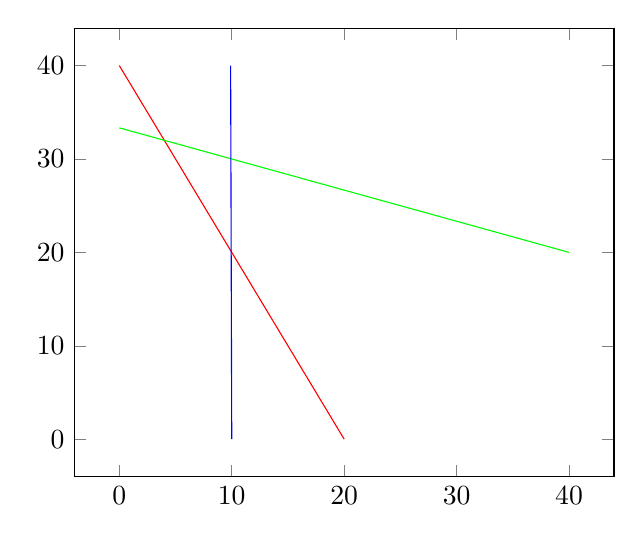
\begin{tikzpicture}
        \begin{axis}
            \addplot[domain=0:20,smooth,red] {40-2*x};
            \addplot[domain=0:40,smooth,green]{100/3-x/3};
            \addplot[domain=9.9:10,smooth,blue] {400*(10-x)};
        \end{axis}
    \end{tikzpicture}
\end{center}
We will be raising $b$ for the line $x_2=-\frac{3}{2}x_1+b,$ until we reach the optimal profit. Note that it is a fact that the \bluebf{feasible region} of solution in a convex polygon. 

It is also a fact that \textbf{if} an optimal solution to a linear programming problem exists, then at least one optimal solution is a \textbf{vertex} of the feasible region.

Now consider if the farmer can plant three crops. Then, each constraint is a plane, and the feasible region will be a convex 3D polygon. For $n$ crops, there will be an exponential number of vertices. 

The simplex method looks at a vertex and all its neighbors. Once we find a vertex that is a local optimum, it will be a global optimum (because of convexity of the feasible region). In the worst case, the simplex method is exponential in the number of variables, but in practice it is very fast. There are now algorithms that can solve linear programming problems in polynomial time (not easy).

\redbf{Optimal Solutions may not exist when:}\begin{enumerate}
    \item The problem is overconstrained (feasible region is empty i.e. $x<0\land x>0$).
    \item The problem is underconstrained (unbounded i.e. $x_1+x_2$ for $x_1,x_2\geq 0$).
\end{enumerate}
\subsection{Integer Linear Programming}
\begin{itemize}
    \item In \bluebf{integer linear programming}, the variables $x_1,\dots,x_n\in\Z.$
    \item In \bluebf{$0$-$1$ LP}, the variables $x_1,\dots,x_n\in\{0,1\}.$ Note that two additional constraints on top of integer linear programming ($x_u\leq1\land x_u\geq0$) will gives us $0$-$1$ LP.
    \item The decision variants of ILP and $0$-$1$ LP are NP-hard. They are much harder than ordinary LP.
    \item Consider the Min Vertex Cover problem for $G=(V,E)$. It can be formulated as a $0$-$1$ LP problem with \begin{itemize}
        \item Variables: $x_u\in\{0,1\},\forall u\in V$
        \item Objective function: $\sum_{u\in V}x_u.$
        \item Constraints: $x_u+x_v\geq 1$ for all $(u,v)\in E.$
    \end{itemize}
\end{itemize}
\section{Complexity and NP-Completeness}
\begin{itemize}
    \item We consider an algorithm to be efficient if it runs in polynomial time in the size of the input.
    \item What if you must solve a problems that there are no algorithms that can solve it in polynomial time?
    \item There is a large set of well-known problems such that \begin{itemize}
        \item Many people have tried to solve efficiently but failed.
        \item If you can solve any one of these problems in polynomial time, you can solve all of them in polynomial time.
    \end{itemize}
    \item This set of problems is called \bluebf{NP Complete}. Our goal is to determine if a problem is NP complete, and to prove problems are NP complete.
    \item The key tool for proving NP completeness is \bluebf{reduction}. A reduction is a way to transform one problem into another. If we can show that one problem is NP complete by reducing it to another problem, then we have shown that the other problem is NP complete.
    \item This is useful because if you are able to prove that a problem is NP complete, you may stop trying to solve it efficiently and look for alternatives (like approximation algorithms).
    \item To illustrate the key concepts, definition, and techniques we will use two \bluebf{decision problems}.
\end{itemize}

\begin{itemize}
    \item Consider the \bluebf{clique} problem. Given a graph $G=(V,E)$, and an integer $k,$ is there a subset $S\subseteq V$ such that $S$ is a clique of size $k.$
    \item The Brute force algorithm is to generate every subset $S\in\mathcal P(V)$ and check if it is a clique. This is exponential in the size of the input as there are $2^{|V|}$ subsets.
\end{itemize}
\begin{itemize}
    \item The \bluebf{Conjunctive Normal Form} (CNF) is a boolean formula consisting of \begin{itemize}
        \item Boolean variables $x_1,\dots,x_n$.
        \item Their negations $\bar x_1,\dots,\bar x_n$.
        \item A literal is a variable of its negation.
        \item A clause $C=l_1\lor l_2\lor\dots\lor l_r$ is a disjunction of literals.
        \item A CNF formula is a conjunction of clauses $\varphi = C_1\land C_2\land\dots\land C_m.$ 
    \end{itemize}
    \item A $k$-CNF formula is a CNF formula with exactly $k$ literals in each clause.
    \item A CNF formula is satisfiable if there is a truth assignment (T/F) to each variable $x_i$ under which $\varphi$ evaluates to true. izz.e. under which each clause of $\varphi$ has at least one literal that evaluates to true.
    \item The $3$SAT problem asks if an input $3$CNF formula $\varphi$ is satisfiable. 
\end{itemize}

\begin{itemize}
    \item So SAT is polynomially reducible to clique if we can transform any given CNF formula $\varphi$ in polynomial time into a graph and an integer $(G,k)$ such that $\varphi$ is satisfiable \redbf{if and only if} $G$ has a clique of size $k.$
    \item If we can show this, then that means if we can solve clique in polynomial time, then we can solve SAT in polynomial time.
    \item The contrapositive is if we cannot solve SAT in polynomial time, then we cannot solve clique in polynomial time.
    \item For the reduction, we can choose $k$ to be the number of clauses. Then, we can construct a graph with one node for every literal of every clause of $\varphi.$ With no edge between nodes in the same clause. An edge between two every pair of nodes representing literals that are compatible. We claim that $\varphi$ is satisfiable iff $G$ has a clique of size $k.$
    \item Suppose $\varphi$ is satisfiable. Then, each clause has a literal that is true. Every pair must be compatible, meaning that they are not both true or both false. So, every pair of literal represents an edge in the graph, so that is a clique of size $k$ in $G$.
    \item Suppose $G$ has a clique of size $k.$ Then, each of the $k$ nodes belong to different clauses. Set these $k$ nodes to be true, then at least one literal in each clause is true. So, $\varphi$ is satisfiable.
    \item The hamiltonian cycle problem, partition problem are all decision problems.
    \item An \bluebf{optimization problem} is stronger than a decision problem. However, it is usually not too much more difficult.\begin{itemize}
        \item For clique, an optimization problem is to find a clique of maximum size.
        \item A harder optimization problem is to find the clique of maximum size that is a subgraph of a given graph.
        \item We claim that if we can solve the decision problem of clique in polynomial time, then we can solve the optimization problems of clique in polynomial time.
    \end{itemize}
\end{itemize}
\subsection{Polynomial Time Reductions}
\begin{definition}[(Karp)]
    $A$ is \bluebf{polynomially reducible} to $B$ denoted $A\leq_pB$ if we can transform any instance of $x$ of $A$ into an instance of $y$ of $B$ in polynomial time such that $x$ is a yes instance of $A$ iff $y$ is a yes instance of $B.$
\end{definition}
\begin{definition}[(Cook)]
    $A\leq_pB$ if, given an oracle for solving $B$ we can solve $A$ in polynomial time by using the oracle polynomially many times.
\end{definition}
\begin{theorem}
    If $A\leq_pB$ and $B$ can be solved in polynomial time, then $A$ can be solved in polynomial time.\begin{proof}
        To solve any instance $x$ of $A,$ we can transform $x$ to $y$ with the same answer than solve instance $y$ of $B$ and return the yes or no answer. The transformation takes polynomial time, and the solution of $B$ takes polynomial time, so the solution of $A$ takes polynomial time.
    \end{proof}
\end{theorem}
\begin{itemize}
    \item Intuitively: A decision problem has an efficient verifier if every yes instance $x$ of $P$ has a short ``justification'' that can be used to efficiently verify that $x$ is indeed a yes instance of $P.$
    \item Consider the SAT problem. If someone claims that a given CNF formula $\varphi$ is satisfiable, then they provide a truth assignment to each variable. This can be verified in polynomial time.
    \item Consider the clique problem with and someone claims that a given graph has a clique of size $k.$ Then, if they provide a set of $k$ nodes, then we can verify that this is a clique in polynomial time.
\end{itemize}
\begin{definition}[Efficient Verifier]
     A decision problem $P$ has an \bluebf{efficient verifier} if there is a polynomial-time verifier algorithm $V(*,*)$ such that \begin{enumerate}
        \item $\forall$ yes instances $x$ of $P,~\exists$ a justification $y$ of polynomial size in the size of $x,$ such that $V(x,y)$ returns yes.
        \item $\forall$ no instances $x$ of $P,$ running the verifier $V(x,y)$ returns no $\forall y.$ 
     \end{enumerate}
     Note that justification is also called ``witness'', ``certificate'', or ``advice''.
\end{definition}
\begin{itemize}
    \item Note that any decision problem that can be solved in polynomial time has an efficient verifier (the trivial verifier, that requires no justification).
    \item For example $s$-$t$ connectivity of an undirected graph $G=(V,E).$ A polynomial time verifier discards the justification and runs BFS starting from $s.$ If the search reaching $t$ then we return yes, otherwise return no.
    \item Note that some decision problems \redbf{may not} have an efficient verifier.
    \begin{itemize}
        \item Consider the complement of Clique (we call ``Clique-Freedom'') problem. Given a graph $G=(V,E)$ and an integer $k,$ does $G$ not have a clique of size $k$? It is non-trivial to design an efficient verifier. We actually don't know if one exists.
        \item Consider the complement of SAT (UNSAT) i.e. given a CNF formula $\varphi,$ does $\varphi$ not have a truth assignment under which it evaluates to true? Or equivalently tautology (does all truth assignments satisfy $\varphi$). We don't know if an efficient verifier exists.
    \end{itemize}
\end{itemize}
\begin{definition}[P,NP,NP-Complete]
    We will use ``efficient/efficiently'' to describe polynomial in the input size.
    \begin{itemize}
        \item $\mathrm{P}$ is the set of decision problems that can be solved efficiently.
        \item $\mathrm{NP}$ is the set of decision problems that have an efficient verifier. We know $\mathrm{P}\subseteq\mathrm{NP}.$
        \item $\mathrm{NP-hard}$ is set of problems such that if a problem $P\in\mathrm{NP-hard}$ then $\forall P'\in\mathrm{NP},~P'\leq_pP.$ Intuitively, $P$ is at least as hard to solve as any problem in $\mathrm{NP}$ because if you can solve $P$ in polynomial time then you can solve \textbf{every} problem in NP in polynomial time.
        \item $\mathrm{NP-Complete}$ is the intersection of $\mathrm{NP}$ and $\mathrm{NP-hard}.$ It is not obvious that $\mathrm{NP-Complete}$ is a non-empty.
    \end{itemize}
\end{definition}
\begin{itemize}
    \item The Cook-Levin Theorem states that SAT is $\mathrm{NP-Complete}.$ As a corollary, we know that if SAT$\notin\mathrm{P}$ then $\mathrm P\neq\mathrm{NP}.$ Otherwise, $\mathrm{P}=\mathrm{NP}.$
    \item Since there are thousands of well-known NP-complete problems that no one has been able to solve in polynomial time, most people believe that SAT$\notin\mathrm{P}.$
    \item As we show that SAT is reducible to clique, by Cook-Levin we know that $\forall P\in\mathrm{NP},~P\leq_p$SAT$\leq_p$Clique. We also show there is an efficient verifier for clique, so clique is NP-complete.
    \item Note that we proved that clique is NP-hard by reducing a known NP-hard problem to it. This is much easier than proving it from scratch.
    \item If you suspect a problem $P$ cannot be solved efficiently, then \begin{enumerate}
        \item See if $P$ is one of the known NP-complete problems.
        \item Try to prove $P$ is NP-hard by finding one of the known NP-complete problem $P'$ and show that $P'\leq_pP.$ 
    \end{enumerate}
    \item We will do many reductions to both expand our list of known NP-complete problems and help us gain experience with reductions.
\end{itemize}

\end{document}